\documentclass[12pt]{article}
\usepackage{graphicx}
\usepackage{float}
\usepackage{grffile}
\usepackage{color}
\usepackage{soul}
\usepackage{tabularx}
\usepackage{multirow}
% use \xspace to allow for space after a macro as necessary
\usepackage{xspace}
\usepackage[top=1in, bottom=1in, left=1.25in, right=1.25in]{geometry}
\usepackage{pdfpages}
\usepackage{lineno}
%% maxwidth is the original width if it is less than linewidth
%% otherwise use linewidth (to make sure the graphics do not exceed the margin)
\makeatletter
\def\maxwidth{ %
  \ifdim\Gin@nat@width>\linewidth
    \linewidth
  \else
    \Gin@nat@width
  \fi
}
\makeatother

\definecolor{commentcol}{rgb}{0.345, 0.345, 0.945}
\newcommand{\comment}[1]{\textcolor{commentcol}{[[#1]]}}%

% general-purpose mathrm macros
\newcommand{\symsub}[2]{\ensuremath{#1_{\tiny \mathrm{#2}}}\xspace}
\newcommand{\mrm}[1]{\ensuremath{\mathrm{#1}}
\xspace}

\usepackage{framed}
\makeatletter
\newenvironment{kframe}{%
 \def\at@end@of@kframe{}%
 \ifinner\ifhmode%
  \def\at@end@of@kframe{\end{minipage}}%
  \begin{minipage}{\columnwidth}%
 \fi\fi%
 \def\FrameCommand##1{\hskip\@totalleftmargin \hskip-\fboxsep
 \colorbox{shadecolor}{##1}\hskip-\fboxsep
     % There is no \\@totalrightmargin, so:
     \hskip-\linewidth \hskip-\@totalleftmargin \hskip\columnwidth}%
 \MakeFramed {\advance\hsize-\width
   \@totalleftmargin\z@ \linewidth\hsize
   \@setminipage}}%
 {\par\unskip\endMakeFramed%
 \at@end@of@kframe}
\makeatother

\definecolor{randomcolor}{rgb}{.97, .27, .67}
\definecolor{shadecolor}{rgb}{.97, .97, .97}
\definecolor{messagecolor}{rgb}{0, 0, 0}
\definecolor{warningcolor}{rgb}{1, 0, 1}
\definecolor{errorcolor}{rgb}{1, 0, 0}
\newenvironment{knitrout}{}{} % an empty environment to be redefined in TeX

\usepackage{alltt}
%% hard to sort by year automatically ...
%% https://tex.stackexchange.com/questions/377449/sorting-citations-and-bibliography-using-natbib-and-plainnat?rq=1
\usepackage[sort]{natbib}
\usepackage{blkarray}
\usepackage{bm}
\usepackage{amsmath,empheq}
\usepackage{alltt}
\usepackage{hyperref}
\usepackage[utf8]{inputenc} % for accented characters
%% stuff for editing
%\usepackage[markup=nocolor,addedmarkup=bf,deletedmarkup=sout]{changes}
%% to suppress notes & comments: \usepackage[final]{changes}
\usepackage{setspace}
\usepackage{changes}
\usepackage[backgroundcolor=lightgray,textsize=tiny]{todonotes}

\bibliographystyle{chicago}
\title{Reformulating phylogenetic mixed models to improve flexibility and speed}
\author{Michael Li and Ben Bolker}
\date{\today}

\providecommand{\keywords}[1]{\textbf{\textit{Keywords:}} #1}
\IfFileExists{upquote.sty}{\usepackage{upquote}}{}
 \vspace{-8ex}
  \date{}
\begin{document}
\newcommand{\dbic}{\ensuremath \Delta \textrm{BIC}}

%% don't typeset BMB comments
\newcommand{\bmbhide}[1]{}
\newcommand{\bmb}[1]{{\color{blue} BB: #1}}


\renewcommand{\figurename}{Fig.}

\newcommand{\mli}[1]{{\color{red} ML: #1}}

\newcommand{\add}[1]{{\color{blue} ADD: #1}}


\newcommand{\pkg}[1]{{\tt #1}}
\newcommand{\code}[1]{{\tt #1}}


% \pagenumbering{gobble}
\linenumbers

% \renewcommand{\bmb}[1]{\relax}
% \renewcommand{\mli}[1]{\relax}



%\SweaveOpts{concordance=TRUE}
%\SweaveOpts{concordance=TRUE}
% \maketitle

\begin{center}
{\Large
\textbf\newline{Reformulating phylogenetic mixed models to improve flexibility and speed} % Please use "sentence case" for title and headings (capitalize only the first word in a title (or heading), the first word in a subtitle (or subheading), and any proper nouns).
}
% Insert author names, affiliations and corresponding author email (do not include titles, positions, or degrees).
\\
\vspace{2pt}
Michael Li\textsuperscript{1*} and Benjamin M. Bolker\textsuperscript{1,2,3}
\\
\vspace{2pt}
* Corresponding author: Michael Li; lim88@mcmaster.ca
\end{center}
\vspace{5pt}
\textbf{1} Department of Biology, McMaster University, Hamilton, Ontario, Canada
\\
\textbf{2} Department of Mathematics and Statistics, McMaster University, Hamilton, Ontario, Canada
\\
\textbf{3} Institute for Infectious Diseases Research, McMaster University, Hamilton, Ontario, Canada
\\
\bigskip

\doublespacing


\section*{Abstract}

\begin{enumerate}
\item{Phylogenetic comparative methods (PCM) using phylogenetic regression are a powerful technique to explore relationships among related groups of species traits. However, existing procedures may be either insufficiently flexible or too computationally demanding when analyzing large volumes of data.}
\item{We propose an alternative formulation of phylogenetic generalized linear mixed models that is mathematically equivalent to previous approaches, but is more flexible in practice. We have implemented this formulation in two R statistical packages (\pkg{lme4} and \pkg{glmmTMB}).}
\item{Our reformulation of phylogenetic generalized linear mixed models is computationally efficient, operating orders of magnitude faster than existing methods for fitting phylogenetic mixed models.}
\item{Our approach can, in principle, be implemented in any platform for generalized mixed models. Our implementation in \pkg{lme4} and \pkg{glmmTMB} allows users to fit phylogenetic mixed models to a broad range of previously difficult cases (e.g., large data, unbalanced observational designs, complex random effects).}
\end{enumerate}



\keywords{phylogenetic comparative methods, phylogenetic correlation, phyloglmm, species--branch matrix}


\section*{Introduction}

%%% PCM accounts for evolutionary relationships. More people are doing it.
Phylogenetic comparative methods (PCMs) are a powerful technique to explore relationships among related groups of species traits.
Given a known phylogenetic tree, PCMs explore the relationships among species traits or distributions while taking the underlying evolutionary relationships of the species into account; they can be used to control statistically for phylogenetic relationships, to quantify phylogenetic signal (a measure of the dependence among species responses due to their evolutionary relationships) in trait distributions, or both. 

Ever-increasing data collection capabilities (e.g., genomic sequencing, telemetry studies of animal behaviour, or environmental remote sensing), in combination with large-scale synthetic databases of species occurrence and phenotypic traits, are making larger volumes of biological data available over an ever-wider taxonomic range.
Researchers use these data to fit complex models describing species occurrence and traits.
For example, ecologists have used phylogenetic relationships in multi-species models \citep{garland1992procedures, freckleton2002phylogenetic, ord2010adaptation, davies2013phylogenetic}; more recently they have begun to integrate evolutionary considerations in applied ecological studies addressing biodiversity conservation and the effects of climate change \citep{winter2013phylogenetic, santamaria2012evolution, lankau2011incorporating, lavergne2010biodiversity, mace2008evolutionary}.
% \bmb{might be interesting to do some bibliometry, although absolutely not necessary --- i.e. how do numbers of citations of (whatever) increase relative to the overall size of the eco/evo literature? \ldots}

Unlike standard regression-based statistical models, where all of the predictor variables of interest (for example, species traits and environmental covariates) are directly observable,  PCMs using phylogenetic regression use phylogenetic relationships to estimate the unobserved process of trait evolution \citep{felsenstein1985phylogenies, butler2004phylogenetic, hansen2012interpreting}. 
% While evolutionary relationships are biologically important and interesting, they often get neglected in applications and multi-species analyses \citep{bunnefeld2012island, santamaria2012evolution}. 
While a wide range of tools is available for phylogenetic regression, existing procedures may be either insufficiently flexible or too computationally demanding when analyzing large volumes of data.
In such cases, researchers typically search for ways to simplify their analyses: for example, treating species effects as independent, thus neglecting phylogenetic correlations among species responses \citep{bunnefeld2012island}; ignoring degrees of relatedness and treating taxon as a strictly hierarchical description \citep{tella1999habitat}; or neglecting within-species variation \citep{ord2010adaptation}.

In this paper, we propose an alternative method for flexibly and efficiently modeling phylogenetic relationships by extending existing software for fitting mixed effect models. 
This method allows researchers to easily incorporate evolutionary and statistical complexities without sacrificing speed.

\subsection*{Challenges in modeling phylogenetic processes}

Standard statistical regression techniques do not allow for correlations among species responses due to their shared evolutionary history.
Classic phylogenetic regression uses a statistical model in which phylogenetic correlation in the residuals from a regression between two species-level traits arises because the residual variation in the dependent-variable trait evolves along the branches of the phylogeny according to a Brownian-motion evolutionary model \citep{felsenstein1985phylogenies}. 
If in addition the residuals are normally distributed and observed without any additional error (e.g., from other covariates) or within-species variation, Felsenstein's method of phylogenetically independent contrasts  \citep[PICS:][]{felsenstein1985phylogenies, nicolakakis2000forebrain} is sufficient to account for the phylogenetic correlation.
More recent approaches -- including phylogenetic generalized linear mixed models (PGLMM) \citep{ives2011generalized, housworth2004phylogenetic}, Pagel's $\lambda$ \citep{pagel1999inferring}, and Blomberg's $K$ \citep{blomberg2003testing} --- build upon PICs by considering different (non-Gaussian) response distributions and by accounting for evolutionary processes other than Brownian-motion. 
These methods partition residual variation into two components: (1) uncorrelated, or independent, residual variation (observation error or tip variation) and (2) phylogenetic signal (evolutionary process error) \citep{hansen2012interpreting, housworth2004phylogenetic}.
If each species' traits are observed more than once, possibly under different conditions, we can potentially distinguish a third level of variation; in this case, phylogenetic variation and tip variation can both be considered part of the evolutionary process error (which we will call tip variation or intercept-level variation) while the among species residual variation is associated with among observation variation within each species.
%\bmb{This is a good point, well expressed. Does PGLMM lump tip variation and within-species variation, or is this primarily an issue with Blomberg/Pagel? Thinking about Boettiger's critique \cite{boettiger2013is} (don't know if it's been peer-reviewed, we could ask him), which might be resolved if we think explicitly about within-species variation \ldots
%\mli{I think it is more like our simulation test. In Boettiger's example, it is treating sister taxa as different species. So it is using a phylogenetic tree of 8 species instead of 4.}
Although many studies include multiple observations per species, phylogenetic analyses rarely take advantage of such information to partition variability more finely.
Indeed, many existing methods are restricted to single observations per species, requiring users to collapse multiple observations per species to species mean values.
%% REMEMBER TO REVISIT IN DISCUSSION

% Figure \ref{fig:variation} illustrates various forms of variation for three species. 
%Despite having multiple observations per tip taxon (species), a typical part of observational or experimental design, but it is rarely seen: existing platforms are unable to fit multiple observations, or unbalanced design data, or both.
% \bmb{OK, but we should be prepared to support this. Could we construct a table of existing approaches/platforms with their capabilities?}
% 
% \begin{center}
% \begin{figure}[H]
%   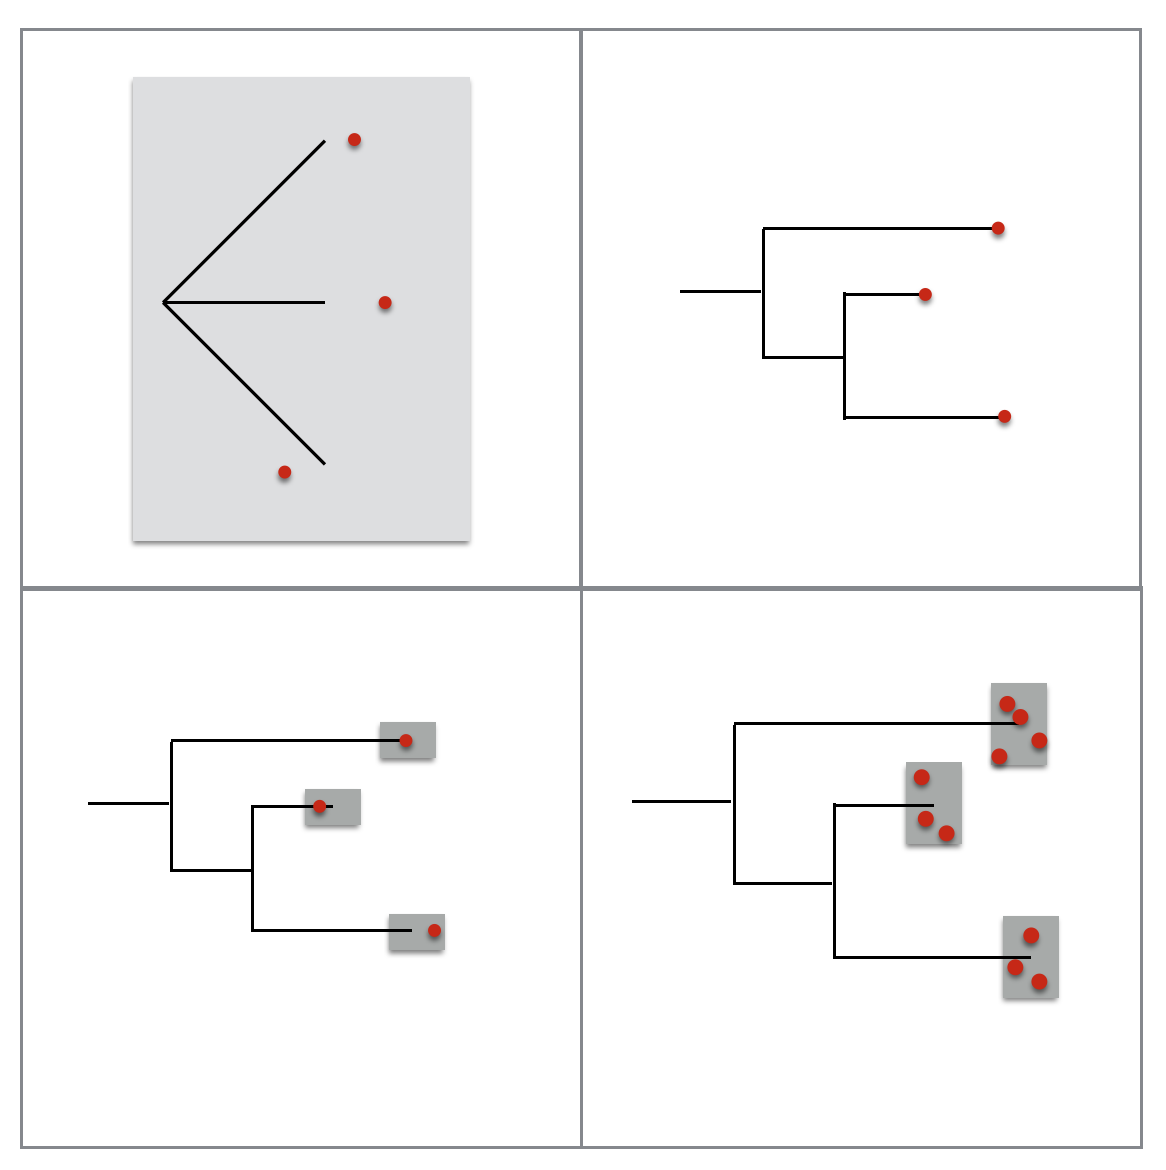
\includegraphics[scale=0.8]{./phylo_diagram.png}
%   \caption{Potential forms of phylogenetic variation of three species. Top left shows pure noise (i.e. assuming a star phylogeny); top right accounts for phylogeny, but without noise; bottom left accounts both phylogeny and noise at the tip, and finally bottom right shows multiple observations (with noise) at the tips.}
% \label{fig:variation}
% \end{figure}
% \end{center}

Classic phylogenetic regressions usually allow the response (trait or distribution) to evolve according to the phylogenetic relationship across species, but the effects of the predictor variables may evolve according to the phylogenetic relationship across species as well. 
For example, suppose we have examined a collection of species that came from two groups, and wish to know whether their brain size (Y) is proportional to their body size (X) (Felsenstein's (1985) example using a mixed-effect model. 
The standard phylogenetic mixed-effect model allows for phylogenetic correlations in the intercept of the relationship between body and brain size. 
However, species within taxonomic groups with similar body sizes may vary in brain size (random intercepts), or taxonomic groups may vary in the relationship between brain and body size (random slopes). 
Analogous to phylogenetically correlated variation in intercepts, phylogenetic random slopes allow the relationship between predictors and responses to vary between species in a phylogenetically correlated way (i.e., similar species will have similar predictor--response relationships).
Several recent studies have incorporated some form of phylogenetic variation using random effects in addition to the standard phylogenetic correlations in the intercepts and looked at species response to phylogenetic variation with changes in environmental factors.
For example, \cite{nowakowski2018phylogenetic} considered phylogenetically correlated slopes in response to habitat conversion when studying the abundance of amphibian species using a Bayesian phylogenetic GLMM, while \cite{li2017canfun} considered phylogenetically correlated species nested within sites when modeling plant abundance via a phylogenetic GLMM approach. 
The tools available for extending phylogenetic relationships to predictor variables (or predictor level variation) in a standard frequentist framework are relatively inflexible; thus, many biologist needing to fit random-slopes model have usually turned to more flexible Bayesian approaches, despite their additional computational burden \citep{hadfield2010mcmc, burkner2018brms}.
Table \ref{table:model} summarizes types of platforms, data constraints, and provides model complexities for phylogenetic comparative analysis.

%% FIXME: chart looks ugly
\begin{table}[]
\begin{tabular}{|l|l|l|l|}
\hline
\textbf{Model} & \textbf{Method} & \textbf{Data} & \textbf{Platform} \\ \hline
\multirow{2}{*}{
\begin{tabular}[c]{@{}l@{}}Generalized Linear \\ Model (GLM)
\end{tabular}} & Correlated residual & Single observation & \begin{tabular}[c]{@{}l@{}}\pkg{nlme}:gls, \\ \pkg{ape}:pic\end{tabular} \\ \cline{2-4} 
& \begin{tabular}[c]{@{}l@{}}Residual \\ + phylogenetic intercept\end{tabular} & Single observation & \begin{tabular}[c]{@{}l@{}}Pagel's $\lambda$\\ Blomberg's $k$ \\ via \pkg{nlme}:gls\\ \pkg{phylolm}\end{tabular} \\ \hline
\multirow{2}{*}{\begin{tabular}[c]{@{}l@{}}Generalized Linear \\ Mixed Model (GLMM)\end{tabular}} & \multirow{2}{*}{Random effect}                                        & \begin{tabular}[c]{@{}l@{}}Single observation\\ Balanced design\end{tabular} & \pkg{pez}                                                                                            \\ \cline{3-4} 
                                                                                                  &                                                                       & Unrestricted                                                                 & \pkg{lme4}, \pkg{glmmTMB}, \pkg{phyr}                                                                                  \\ \hline
\multirow{2}{*}{Bayesian GLMM}                                                                    & \multirow{2}{*}{Random effect}                                        & Balanced design                                                              & \pkg{MCMCglmm}                                                                                       \\ \cline{3-4} 
                                                                                                  &                                                                       & Unrestricted                                                                 & \pkg{brms}                                                                                           \\ \hline
\end{tabular}
\caption{List of phylogenetic generalized linear models and R packages.}
\label{table:model}
\end{table}

In this paper, we will propose an alternative formulation of phylogenetic regression in a generalized linear mixed modeling framework that is mathematically equivalent to previous approaches, but more flexible.
In particular, it easily allows for random effects (such as random intercepts, random slopes, and random interactions), without the need to implement special correlation structures, by incorporating phylogenetic structures as part of the mean model \citep{hefley2017basis}.
%% can be incorporated relatively easily into any mixed-model platform that allows new random-effects design matrices to be specified, and can be easily extended along with the features of mixed model such as multiple observational designs, phylogenetic random-slopes models, and multiple (nested or crossed) random effects.
We will compare our technique coded in R packages \pkg{lme4} and \pkg{glmmTMB} with existing R packages (i.e. \pkg{nlme} \citep{pinheiro2014r}, \pkg{phylolm} \citep{ho2014phylolm}, \pkg{pez} \citep{pearse2015pez} \pkg{phyr} \citep{phyr}, \pkg{MCMCglmm} \citep{hadfield2010mcmc}, and \pkg{brms} \citep{burkner2018brms}), fitting models to data from simulated model that incorporates phylogenetic variation from both predictors and tips/species as well as residual variation.
% We expect that our approach will be fast as well as flexible, because \pkg{lme4} and \pkg{glmmTMB} use efficient approaches. 
%% TODO LAST LINE SEE PAGE 5

%% FIXME: move to methods/simulations
% In principle, for any given valid method that matches the simulation model should eventually converge to the simulated parameters. 
% We end by discussing opportunities and practicalities of our method and comments on the state of art for this area of research. 

\section*{Materials and Methods}

\newcommand{\bX}{{\mathbf X}}
\newcommand{\bbeta}{{\boldsymbol \beta}}
\newcommand{\bmu}{{\boldsymbol \mu}}
\newcommand{\bY}{{\mathbf y}}  %% fixme later
\newcommand{\bC}{{\mathbf C}}
\newcommand{\bZ}{{\mathbf Z}}
\newcommand{\bb}{{\mathbf b}}
\newcommand{\besp}{{\boldsymbol \epsilon}}
\newcommand{\bSigma}{{\boldsymbol \Sigma}}

We generated test data using a simple framework that combines fixed effects, phylogenetic random intercept, slope, and their correlations from a phylogenetic tree, as well as residuals. 
We then fit the test data from these simulations using our approach implemented using the R packages \pkg{lme4} \citep{bates2015fitting} and \pkg{glmmTMB} \citep{brooks2017glmmTMB}, using assumptions that match those of the simulation model. We also fit with other platforms, using standard simplifications when necessary for implementation.

\subsection*{Phylogenetic regression}

We begin by describing the classic phylogenetic regression in a linear regression setting.
Consider a simple linear regression model of observable trait $\bY$ as a function of some predictors encoded in a model matrix $\bX$, where each species is measured exactly once. 
The standard phylogenetic regression can be formulated as

%\bmb{boldface matrices/vectors i.e. $\bX \bbeta$? or not worth the trouble? How about $\bmu=\bX \bbeta$; $\bY \sim \textrm{MVN}(\bmu,\sigma^2 \bC)$ for greater generality? (OK, I see that you move in this direction later.  But I'm not sure it's worth the detour of using two different notations? even if you are going to extend to include fixed effects, $Z$, etc. later ...}:

\begin{equation}
\begin{aligned}
\bY & = \bX \bbeta + \besp  \\
\besp & \sim \textrm{MVN}(0,\sigma^{2} \bC), 
\label{eq:gls}
\end{aligned}
\end{equation}
where $\bY$ is an $n \times 1$ response vector; $\bX$ is an $n \times m$ model matrix, describing $n$ observations of $m$ predictor variables (phenotypic traits or environmental variables, typically including an intercept column of ones); $\bbeta$ is an $m$-vector of coefficients; $\besp$ is an $n \times 1$ vector which is assumed to be multivariate normally distributed with mean $0$ and variance-covariance matrix given by $\sigma^{2} \bC$ where $\bC$ is a $n \times n$ phylogenetic covariance (PC) matrix.
The PC matrix is inferred from the topology of the evolutionary tree by quantifying the degree of shared evolution between any pair of taxa \citep{garamszegi2014modern}.

%\bmb{give a ref for this? maybe Paradis's ape book, or Garamszegi's book, or ?}
%\mli{chapter 7 in garamszegi 2014}

% More recently, researchers use linear mixed model and generalized linear mixed model framework to model complex systems with phylogenetic structures.
%\mli{Why? Data type, interactions, random effects, etc... Need to really explain random effects here. Alternatively, we can drop this line and write this...}

\subsection*{Phylogenetic generalized linear mixed model}
Alternatively, one can use the generalized linear mixed effects modeling (GLMM) framework to define a wider range that includes the standard phylogenetic regression as a special case \citep{lynch1991methods}.
The generalized linear mixed effect model allows for non-Gaussian responses and uses random effects to flexibly incorporate multiple types of variability.
The typical GLMM has the form:
\newcommand{\dist}{{\cal D}}
\begin{equation}
\begin{aligned}
\bY & = \dist(g^{-1}(\bmu), \phi) \\
\bmu & = \bX \bbeta + \bZ \bb  \\
\bb & \sim \textrm{MVN}(0, \bSigma(\theta))  \\
\label{eq:glmm}
\end{aligned}
\end{equation}
where $\bZ$ is an $n \times q$ model matrix for the $q$-dimensional vector-valued random effects variables; $\bb$ (sometimes referred to as the ``G-side" effect) representing the conditional mean (or mode) of the random effect, which is assumed to be multivariate normally distributed with a variance-covariance matrix given by $\bSigma(\theta)$; and $\phi$ is a scale parameter for the conditional distribution $\dist$.
When $\dist$ is Gaussian, $g$ is the identity function, $\bZ$ is the identity matrix, and $\bSigma(\theta)=\sigma^2\bC$, (\ref{eq:glmm}) reduces to (\ref{eq:gls}).
% ; $\besp$ (sometimes referred as "R" effect) is an $n \times 1$ vector of independent and normally distributed error terms with variance $\sigma_{\epsilon}^2$.
% Analogously, the phylogenetic regression given by (\ref{eq:gls1}) can be represented in the generalized mixed model framework with Gaussian responses by constraining $\bSigma(\theta) = \sigma^2 \bC$ and $\sigma^{2}_{\epsilon} = 0$.

%% Check if the two s. above make sense.

%%MLi: The P below does not feel like it belongs here. 
% There are several forms of random variation in the mixed model framework.
% First, random intercepts can allow the response trait to vary independently across groups other than species (e.g., patches, sites, or experiments). 
% Second, random intercepts can also allow the response (trait or distribution) to vary either independently among species (since species represent the tips of the phylogenetic tree) or among species in a phylogenetically correlated way (i.e., species that are closely related tend to have similar responses).
% The third type of variation are random slopes; they allow fixed effects (the relationship between predictors and responses) to vary among groups.

% \bmb{worth including the \pkg{MCMCglmm}/\pkg{brms} inverse-VCV formulation here? And/or contacting Eric Pedersen to find out about his Markov Random Field phylog. stuff in GAM?}
% \mli{inverse VCV for BLUP? an alternative way to find the inverse of the vcv(phy)}
% \mli{G vs R, PIC and simple variations (phylolm ...) uses R and no G}

\subsection*{Reformulating the phylogenetic covariance matrix}
% The standard problem of phylogenetic comparative methods is to analyze relationships among data where the observations are gathered from nodes (usually tips) of a phylogenetic tree.
% Phylogenetic independent contrasts is a generalization of the paired comparisons method where contrasts are taken for each bifurcation (nodes) in a phylogenetic tree. 
% Assuming that traits evolve independently in each lineage following speciation, then the trait divergences that occur at one node are independent of divergence at other nodes.  


\newcommand{\bS}{{\mathbf S}}
\newcommand{\bJ}{{\mathbf J}}
\newcommand{\bB}{{\mathbf B}}
\newcommand{\bBadj}{{\mathbf B}_{\mbox{\tiny adj}}}
\newcommand{\bomega}{{\boldsymbol \omega}}
\newcommand{\bell}{{\boldsymbol \ell}}
\newcommand{\e}{{ \epsilon}}

The duality of $\bSigma$ and $\bZ$ for equivalent model specifications is useful for efficient implementations of models that contains a functional covariance structure \citep{hefley2017basis}. 
Similarly, we can construct phylogenetic correlations (PC) through $\bZ$.
Suppose that the evolution follows a Brownian-motion process, i.e., continuous traits evolve independently, following an unbiased, continuous-time random walk, along each branch of the phylogeny.
In this case, the phylogenetic variability of a particular species can be written as the sum of the variances of evolutionary changes that occurred on all of the branches in its history. 
Thus, modeling the evolutionary history of each species with a sequence of independent errors with species--branch matrix $\bS$ is equivalent to imposing a correlation $\bC$.
For example, for the phylogeny in figure \ref{fig:tree}, the corresponding $\bS$ takes the form:

%% FIXME: need top/side labels
\begin{center}
\begin{figure}[H]
  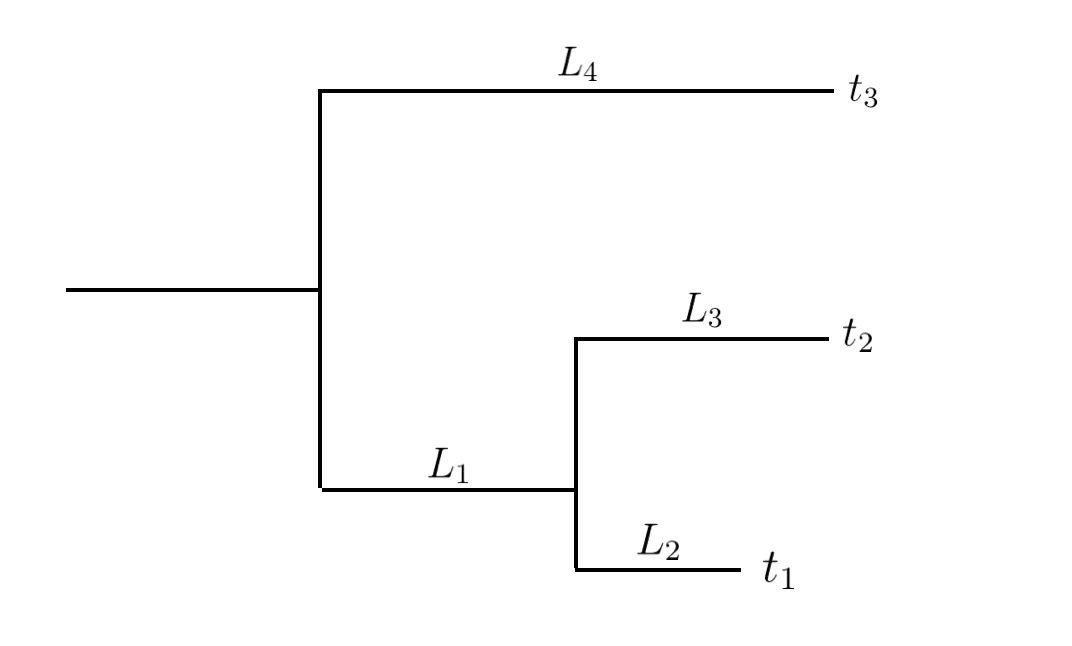
\includegraphics[scale=0.8,page=1]{./figure/phylotree.png}
  \caption{Three-species phylogenetic tree.}
\label{fig:tree}
\end{figure}
\end{center}
\[
  \begin{blockarray}{ccccc}
  & L_1 & L_2 & L_3 & L_4  \\
  \begin{block}{c(cccc)}
  t_1 & \ell_1 & \ell_2 & 0           & 0 \\
  t_2 & \ell_1 &  0          & \ell_3 & 0 \\
  t_3 & 0           &  0          & 0           & \ell_4 \\
  \end{block}
  \end{blockarray}
  \hspace{0.5cm}
  \begin{blockarray}{(c)}
  \e_1 \\
  \e_2 \\
  \e_3 \\
  \e_4 \\
  \end{blockarray}
  \]
% \begin{pmatrix}
% \e_1 \\
% \e_2 \\
% \e_3 \\
% \e_4
% \end{pmatrix}
%% FIXME: double check this
The phylogenetic variability corresponding to species 1 is $\ell_1 \e_1 + \ell_2 \e_2$, where $\ell_i = \sqrt{L_i}$, the square root of the branch length $L_i$ in figure \ref{fig:tree}, and the $\e_i$ are independent Normal variates with zero mean and $\sigma^2$ evolutionary variance (i.e. the variance for species 1 is $\textrm{E}[(\ell_1 \e_1 + \ell_2 \e_2)^2] = (L_1 + L_2)\sigma^2$).
% The variance of Brownian-motion, is the evolutionary rate, where it is linear in evolution time.

\subsubsection*{Constructing the species--branch random effects model matrix}

The $\bS$ matrix is the product of an $m \times b$ indicator matrix $\bS_{ind}$ of branch indices and a vector $\bell$ of square roots of branch lengths:

\[
\bS_{ind} = \begin{bmatrix}
1 & 1 & 0 & 0 \\ 
1 & 0 & 1 & 0 \\ 
0 & 0 & 0 & 1
\end{bmatrix} , 
\qquad
\bell = \begin{bmatrix}
\ell_1 \\
\ell_2 \\
\ell_3 \\
\ell_4 
\end{bmatrix} .
\]
$\bS_{ind}$ is a binary (indicator) matrix that describes whether a particular branch occurs in the history of a focal species. 
$\bS \bS^T$ gives the variance-covariance matrix of the phylogeny. 

In general, the random-effect model matrix $\bZ$ for a GLMM can be decomposed into term-wise model matrices $\bZ_{i}$ as described in \citet{bates2015fitting}.
Analogous to the procedure described in \citet{bates2015fitting}, the phylogenetic correlated random-effect matrix $\bZ^{C}_{i}$ is

\begin{equation}
\bZ^{C}_{i} = (\bS^{\top}\bJ^{\top}_{i} \ast \bX^{\top}_{i})^{\top}, \label{eq:ZC}
\end{equation}
where $\bS$ is the $m \times b$ species--branch matrix; $\bJ_{i}$ is the $n_i \times m$ indicator matrix of grouping factors; $\bX_{i}$ is the $n \times p_{i}$ raw random-effects model matrix; and $\ast$ is the Khatri-Rao product \citep{khatri1968solutions} partitioned at the observation level ($n$).

For example, using the phylogeny above (figure \ref{fig:tree}), if we begin with a raw model matrix corresponding to a random-slope model, 

\[
\bX = \begin{bmatrix}
1 & t_1  \\ 
1 & t_2  \\ 
1 & t_3 
\end{bmatrix} 
\]
then the term-wise phylogenetic random effects model matrix is,

\begin{equation}
\begin{aligned}
\bZ^{C}_{i} = (\bS^{\top}\bJ^{\top}_{i} \ast \bX^{\top}_{i})^{\top} =
\left[
\left(
\begin{bmatrix}
\ell_{1} & \ell_{1}  & 0 \\
\ell_{2} &  0  & 0 \\
0  &  \ell_{3} & 0 \\
0 & 0 &  \ell_{4} 
\end{bmatrix}
\begin{bmatrix}
1 & 0  & 0 \\
0 & 1  & 0 \\
0 & 0  & 1  
\end{bmatrix}
\right)
\ast
\begin{bmatrix}
1   & 1   & 1  \\ 
t_1 & t_2 & t_3
\end{bmatrix} 
\right]^{\top}
\\
= \begin{bmatrix}
\ell_{1} & \ell_{1}t_1 & \ell_{2} & \ell_{2}t_1 & 0 & 0 & 0 & 0 \\
\ell_{1} & \ell_{1}t_2 & 0 & 0 & \ell_{3} & \ell_{3}t_2 & 0 & 0 \\
0 & 0 & 0 & 0 & 0 & 0 & \ell_{4} & \ell_{4}t_3
\end{bmatrix}.
\end{aligned}
\end{equation}


% 
% The scaled species--branch matrix $\bS_{adji}$ is scaled version of $\bS$ via the standardized generalized variance (SGV).
% SGVs are used as an intrinsic/natural way to scale down the variance-covariance matrix measured in different scales (for example, phylogenetic distance, years and etc) compariable to other variation in the model \citep{sengupta1987tests}.
% SGV is the $nth$ root of the generalized variance (GV), or the determinant of the variance-covariance matrix, where GV measures the overall size or volume of the variance-covariance matrix.  
% The SGV is given by:
% \begin{align}
% \bomega & = \textrm{det}(\bSigma_{phy})^{1/n},
% \end{align}
% where $n$ is the number of species in the phylogeny.
% 
% The analog in the $\bS$ is to scale the branch vector $\bell$ by square root of the SGV:
% \begin{align}
% \bell_{adj} & = \frac{\bell}{\sqrt{\bomega}}
% \end{align} 
% and the $\bS_{adj}$ is the matrix product of $\bS_{ind}$ and $\bell_{adj}$.

\subsection*{Simulation}
\subsubsection*{Single group model}

We generated test data based on the random slopes mixed model formulation (\ref{eq:glmm}) with a single response variable $\bY$ and a single continuous normally distributed predictor variable $\bm{t}$ for $n$ = 25, 50, and 100 species.
For simplicity, the response variable $\bY$ is conditionally normally distributed (i.e., $\cal{D}$ is a Gaussian distribution, and $g$ is the identity link function), corresponding to a linear mixed effect model. 
For the first set of simulations, we simulate one observation per species.
% For a broader range of comparisons, we simulate one observation ($X_i,Y_i$) per species.
Thus, the full simulation model is as follows:
\begin{equation}
\begin{aligned}
\bY & = \dist(g^{-1}(\bmu), \phi) \\
\bmu & = (\bf{\beta_0 + b_{\mathrm{phy_{int}}}}) + (\bf{\beta_1 + b_{\mathrm{phy_{slope}}}}) \bm{t} + \besp \\\
(\bf{b_{\mathrm{phy_{int}}}, b_{\mathrm{phy_{slope}}}}) & \sim \textrm{MVN} \left( 0, \begin{bmatrix}
\Sigma^2_{\mathrm{phy_{int}}} & \Sigma_{\mathrm{phy_{int-slope}}} \\ 
\Sigma_{\mathrm{phy_{int-slope}}} & \Sigma^2_{\mathrm{phy_{slope}}}
\end{bmatrix} 
\right) \\ 
\besp & \sim \textrm{N} ( 0 , \sigma_{\epsilon}^2) .
\label{eq:single_glmm}
\end{aligned}
\end{equation}
The model contains two fixed effect parameters ($\beta_0$ and $\beta_1$), three random effect parameters (phylogenetic random intercept variance $\Sigma^2_{\mathrm{phy}_{int}}$, phylogenetic random slope variance $\Sigma^2_{\mathrm{phy}_{slope}}$ and covariance between phylogenetic random slope and intercept $\Sigma_{\mathrm{phy_{int-slope}}}$) and residual variance ($\sigma_{\epsilon}^2$).  
The covariance between phylogenetic random intercept and slope measures the correlation of phylogenetic dependency variability in regression effect ($b_{\mathrm{phy_{slope}}}$) and response ($b_{\mathrm{phy_{int}}}$); i.e. if a positive correlation indicates that similar species have similar relative intercepts and slopes.
Predictor-level and intercept-level random effects of species are not applicable in this simulation setting because there is only a single observation per species, so within-species variation cannot be separated from tip variation.

\subsubsection*{Multi-group model}

We extend the simulation model by adding multiple groups where each group has one observation per species. 
The multi-group model is a generalization of multiple-site models used in community ecology to model phylogenetic attraction \citep{helmus2007separating}. 
The full multi-group model is as follows: 
\begin{equation}
\begin{aligned}
\bY & = \dist(g^{-1}(\bmu), \phi) \\
\bmu & = (\bf{\beta_0 + b_{\mathrm{phy_{int}}} + b_{\mathrm{sp_{int}}} + b_{\mathrm{group}}}) + (\bf{\beta_1 + b_{\mathrm{phy_{slope}}} + b_{\mathrm{sp_{slope}}}}) \bm{t} + \bf{b_{\mathrm{sp:group}}} + \besp \\
(\bf{b_{\mathrm{phy_{int}}}, b_{\mathrm{phy_{slope}}}}) & \sim \textrm{MVN} \left( 0, \begin{bmatrix}
\Sigma^2_{\mathrm{phy_{int}}} & \Sigma_{\mathrm{phy_{int-slope}}} \\ 
\Sigma_{\mathrm{phy_{int-slope}}} & \Sigma^2_{\mathrm{phy_{slope}}}
\end{bmatrix}
\right) \\
(\bf{b_{\mathrm{sp_{int}}}, b_{\mathrm{sp_{slope}}}}) & \sim \textrm{MVN} \left( 0, \begin{bmatrix}
\sigma^2_{\mathrm{sp_{int}}} & \sigma_{\mathrm{sp_{int-slope}}} \\ 
\sigma_{\mathrm{sp_{int-slope}}} & \sigma^2_{\mathrm{sp_{slope}}}
\end{bmatrix}
\right) \\
\bf{b_{\mathrm{group}}} & \sim \textrm{MVN} ( 0 , \sigma^2_{\mathrm{group}}) \\
\bf{b_{\mathrm{sp:group}}} & \sim \textrm{MVN} (0, \mathrm{I}_{\mathrm{group}} \otimes \Sigma^2_{phy}) \\
\besp & \sim \textrm{N} ( 0 , \sigma_{\epsilon}^2),
\label{eq:multiple_glmm}
\end{aligned}
\end{equation}
where $\textrm{I}_{\textrm{group}}$ is a indicator matrix of groups; and $\otimes$ is the Kronecker product.

The multi-group full simulation model has five additional random effects (predictor-level ($\sigma^2_{\mathrm{sp_{slope}}}$) and intercept-level ($\sigma^2_{\mathrm{sp_{int}}}$) random effect of species variance and their covariance ($\sigma_{\mathrm{sp_{int-slope}}}$), random intercept of group ($\bf{b_{\mathrm{group}}}$) and random intercept of species-group interaction ($\bf{b_{\mathrm{sp:group}}}$)) compared to the single--group full model.
Predictor-level and intercept-level random effects of species are applicable in the multi-group model setting because there are multiple observations per species; thus we can distinguish variation among species separately from residual variation.
Variance in the intercept of species--group interactions ($\bf{b_{\mathrm{sp:group}}}$) describes whether the species within a group have more similar responses on average than expected by chance, equivalent to phylogenetic attraction \citep{helmus2007separating}. 

\subsection*{Platforms}

We compare our approach with five other R packages that can fit phylogenetic comparative models: \pkg{nlme} \citep{pinheiro2014r}, \pkg{phylolm} \citep{ho2014phylolm}, \pkg{pez} \citep{pearse2015pez}, \pkg{phyr} \citep{phyr} and \pkg{brms} \citep{burkner2018brms}.
% \bmb{I think nlme can do other evolutionary models as well? May not be worth mentioning ...}
% \begin{verbatim}
% grep("\\.",apropos("^cor[A-Z]",ignore.case=FALSE),
% invert=TRUE,value=TRUE)
% \end{verbatim}
Phylogenetic generalized least squares (PGLS) (\code{gls} in \pkg{nlme}) is one of the most widely used techniques in phylogenetic comparative analysis; it fits a linear model where the covariance structure between species assumes an evolutionary process on the tree (typically Brownian-motion, but other processes can be used) instead of treating the residual error for each species as independent.
Phylogenetic generalized linear models (PGLM) (\code{phyloglm} in the \pkg{phylolm} package) are a slightly more flexible variation of PGLS that can allow for both phylogenetic and residual variation, as well as non-Gaussian response variables.
Both \code{gls} and \code{phylolm} can model non-Brownian evolutionary processes and different correlation structures (e.g., Pagel's $\lambda$ or Blomberg's $K$), but we restrict our PGLS fits to the simple BM correlation. 
Neither PGLS nor PGLM can handle random slopes or multiple observations within a species.
One of the few packages that currently fit phylogenetic slopes to predictor level variation is \pkg{pez} (and very recently \pkg{phyr}), which can handle additional random slopes ($\Sigma^2_{\mathrm{phy_{slope}}}$) and random intercepts of species-group interactions ($\bf{b_{\mathrm{sp:group}}}$) but does not incorporate covariation between phylogenetic random slope-intercept ($\Sigma_{\mathrm{phy_{int-slope}}}$).
Lastly, Bayesian phylogenetic GLMMs using Markov chain Monte Carlo (MCMC) can handle all of the cases described above. 
However, MCMC is usually much more computationally expensive for GLMMs than platforms using deterministic optimization.
\pkg{MCMCglmm} \citep{hadfield2010general} is the most widely used Bayesian phylogenetic GLMM, but we will instead use \pkg{brms}, which uses a more computationally efficient MCMC technique called Hamiltonian Monte Carlo (HMC)\citep{duane1987hybrid}.
 
% Table \mli{ref something} provides the statistically equivalent fitting capabilities of common/existing phylogenetic methods.
\begin{table}[]
\resizebox{\textwidth}{!}{%
\begin{tabular}{|c|c|c|c|c|c|c|c|}
\hline
\textbf{Package} & \pkg{nlme} & \pkg{phylolm} & \pkg{lme4}/\pkg{glmmTMB} & \pkg{pez} & \pkg{phyr} & \pkg{brms} & \pkg{MCMCglmm} \\ \hline
Single Group & X & X & X &  &  & X & X \\ \hline
\begin{tabular}[c]{@{}c@{}}Phylo Intercept\\ Phylo Slope\\ Phylo Slope-Intercept correlation\\ Residual\end{tabular} & X & \begin{tabular}[c]{@{}c@{}}X\\ \\ \\ X\end{tabular} & \begin{tabular}[c]{@{}c@{}}X\\ X\\ X\\ X\end{tabular} &  &  & \begin{tabular}[c]{@{}c@{}}X\\ X\\ X\\ X\end{tabular} & \begin{tabular}[c]{@{}c@{}}X\\ X\\ X\\ X\end{tabular} \\ \hline
Multi-group &  &  & X & X & X & X & X \\ \hline
\begin{tabular}[c]{@{}c@{}}Phylo Intercept\\ Phylo Slope\\ Phylo Slope-intercept correlation\\ Phylo Species-group interaction\\ Species intercept\\ Species Slope \\ Species Slope-intercept correlation\\ Residual\end{tabular} &  &  & \begin{tabular}[c]{@{}c@{}}X\\ X\\ X\\ X\\ X\\ X\\ X\\ X\end{tabular} & \begin{tabular}[c]{@{}c@{}}X\\ X\\ \\ X\\ X\\ X\\ \\ X\end{tabular} & \begin{tabular}[c]{@{}c@{}}X\\ X\\ \\ X\\ X\\ X\\ \\ X\end{tabular} & \begin{tabular}[c]{@{}c@{}}X\\ X\\ X\\ X\\ X\\ X\\ X\\ X\end{tabular} & \begin{tabular}[c]{@{}c@{}}X\\ X\\ X\\ \\ X\\ X\\ X\\ X\end{tabular} \\ \hline
\end{tabular}%
}
\caption{List of estimable parameters for each R package.}
\label{table:platform}
\end{table}

\subsection*{Simulation and evaluations}

We simulated 100 random phylogenetic trees using R package \pkg{ape} \citep{ape} for each sample size (n = 25, 50, 100 and an additional n = 500 for the multi-group model) to generate and then modelled responses on each tree using (\ref{eq:single_glmm}, \ref{eq:multiple_glmm}). 
Each realization was fitted using all model variants. 
All simulation parameters are shown in Figure \ref{ssplot} and Figure \ref{msplot}. 
Correlation $\rho_{xy}$ is used in place of covariances $\Sigma_{xy}$ (i.e., $\rho_{xy} = \frac{\Sigma_{xy}}{\Sigma_{x}\Sigma_{y}}$) in the simulations.
Table \ref{table:platform} shows the parameters that are estimable for each platform. 
We only evaluated the goodness of fit for model fits that passed the convergence tests implemented by the package.
For Bayesian GLMM, we included only realizations where we require values of the Gelman-Rubin statistic less than the recommended threshold 1.1. Based on recent concerns about Gelman-Rubin thresholds \citep{vats2018revisiting}), we included the additional convergence criterion of effective sample size (ESS) $>1000$ for the fixed effect parameters ($\beta_{0}$ and $\beta_{1}$) for each replication \citep{vehtari2019rank}. 
For each replication, we sample two chains starting with 10000 iterations. 
We first evaluate our estimates by looking at the distribution of the estimated values (maximum likelihood estimates for non-Bayesian platforms and posterior medians for Bayesian platforms) to quantify bias and variance (i.e., quality of the point estimate).
We then compute frequentist coverage to assess the quality of the confidence intervals.
Coverage refers to the proportion of simulations in which the computed confidence intervals include the true values of parameters.
We used 95\% Wald confidence intervals for deterministic methods and quantile-based intervals (for Bayesian GLMM) to evaluate coverage.
% \bmb{clarify: did you use profile if available, otherwise Wald? You don't give any more detail in your coverage plots. [How different were Wald and profile for these results, or did you not compare them?]}
We also compare computational speed between different platforms to evaluate the efficiency of different platforms and methods. 

\section*{Results}

We used our method to reproduce the examples in chapter 11 of \cite{garamszegi2014modern} using phylogenetic GLMMs based on \pkg{lme4} and \pkg{glmmTMB} (for more details see example in supplement).

\subsection*{Single Group model simulations}

\begin{center}
\begin{figure}[H]
  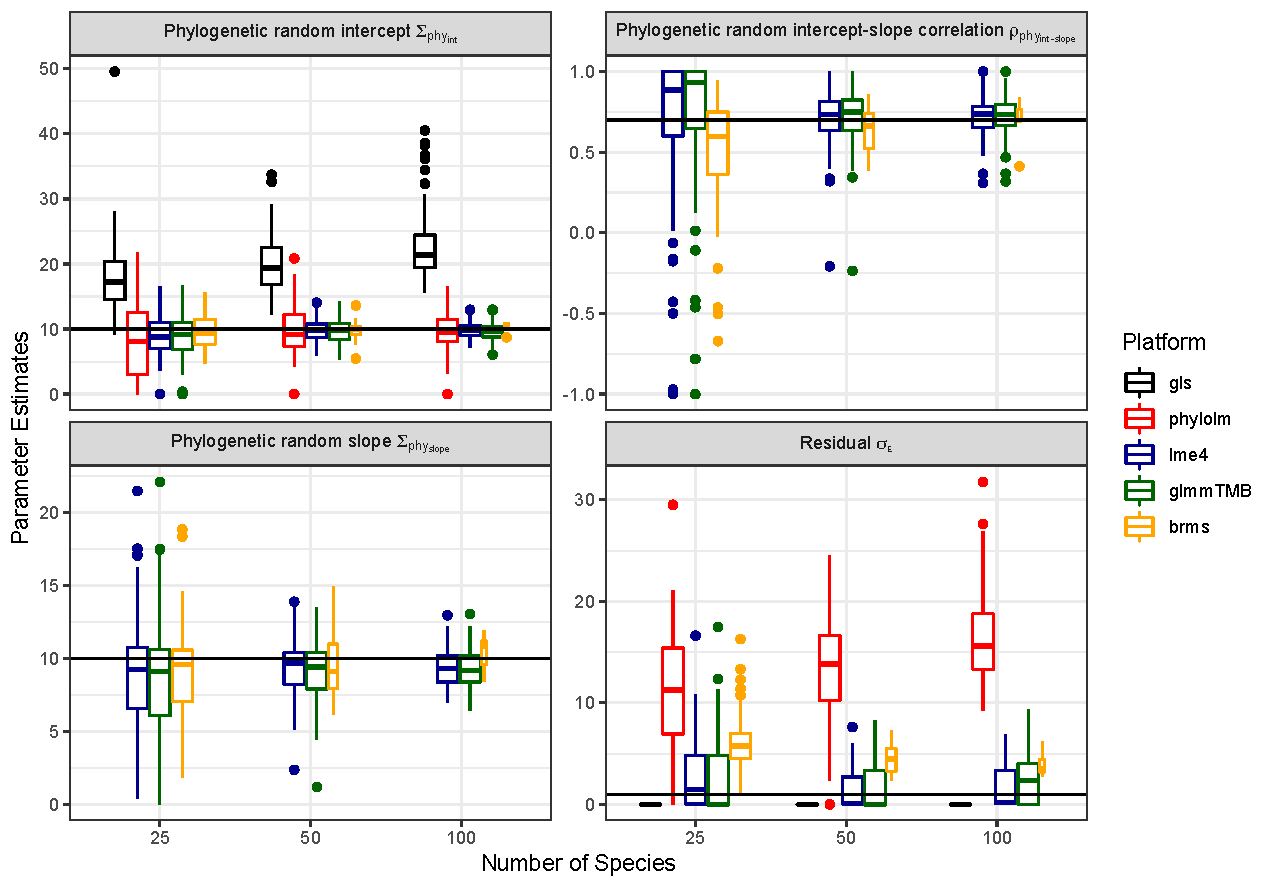
\includegraphics[scale=0.7,page=1]{./figure/ssplot.pdf}
  \caption{Comparison of single group model parameter estimates across different R packages in Table \ref{table:platform}. Total simulations $N=100$ for each category. The horizontal line shows the true value of the parameters in the simulation model. Models capable of fitting all parameters (\pkg{lme4},  \pkg{glmmTMB}, and \pkg{brms}) fit well for all parameters. 
%\bmb{consider tweaking aspect ratio (slightly wider?) Consider including n=25, n=50, n=100 in x-axis tick labels (I don't have all the output data so can't rebuild figs myself ...)
%\jd{Use dashed lines (or some other gg signifier) for the insufficient approaches}
}
\label{ssplot}
\end{figure}
\end{center}
\begin{center}
\begin{figure}[H]
  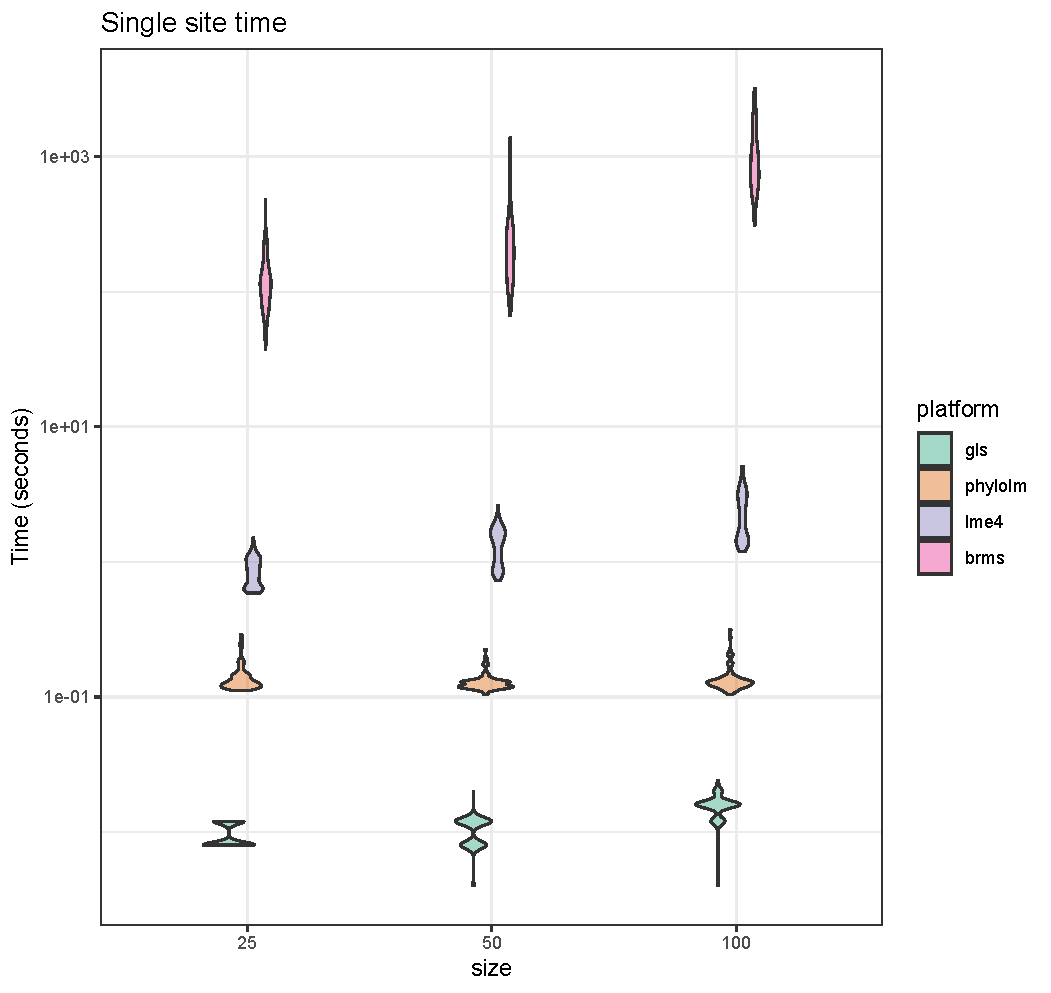
\includegraphics[scale=0.7]{./figure/sstime.pdf}
  \caption{Comparison of single-group model computational speed.}
\label{ssplot_speed}
\end{figure}
\end{center}
\begin{center}
\begin{figure}[H]
  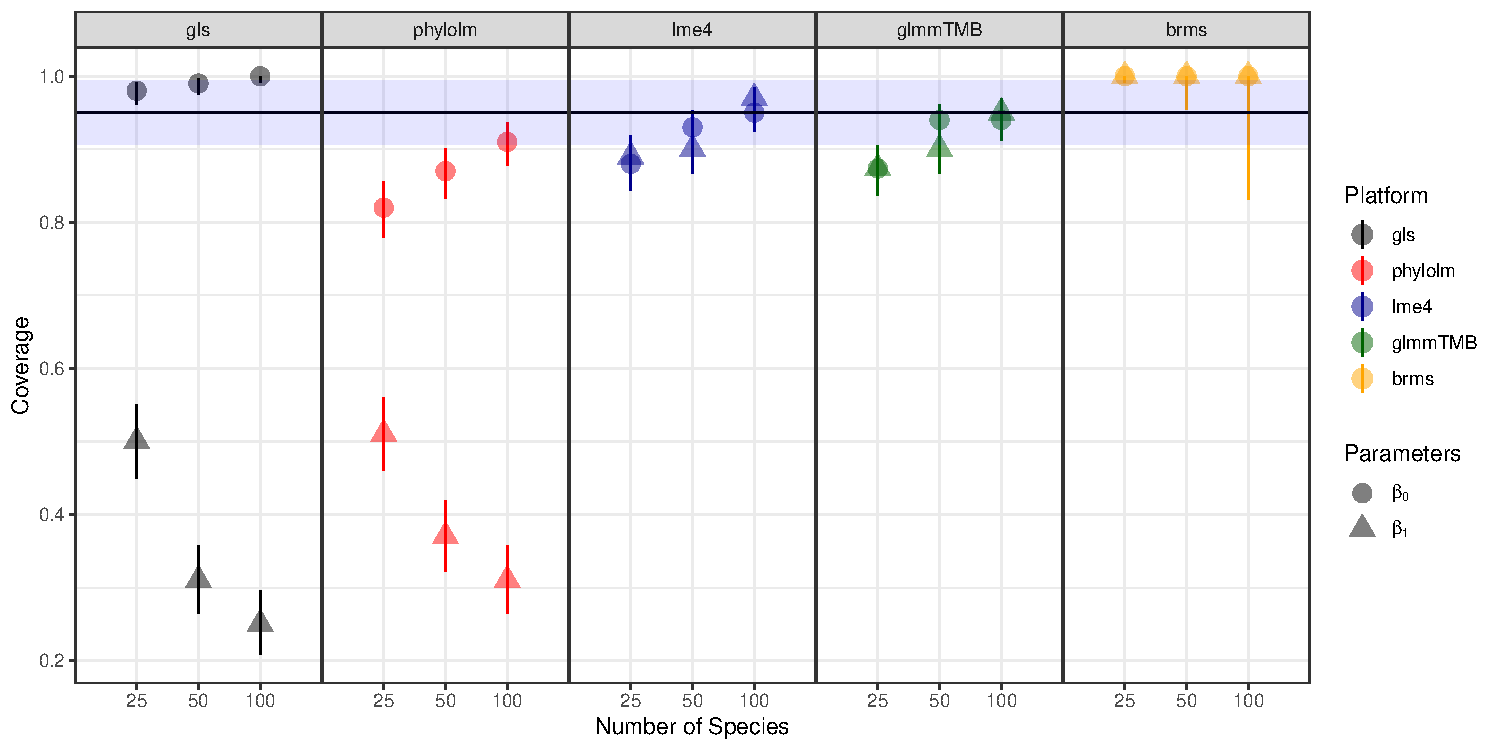
\includegraphics[scale=0.7]{./figure/sscoverage.pdf}
  \caption{Comparison of coverage probability for fixed effect parameters. Models matching the simulation model (\pkg{lme4}, \pkg{glmmTMB} and pkg{brms}) have coverage near the nominal value of 0.95. The black line shows the nominal coverage, and the blue ribbon the 95\% binomial confidence interval based on 100 simulated fits. 
%  \bmb{really picky, but maybe change grid lines or ribbon colour slightly so they're not confusable (maybe use blue ribbon with alpha=0.1?)}
  }
\label{ssplot_coverage}
\end{figure}
\end{center}

The full fitted model (which matches the simulation model that incorporates phylogenetic intercept, slope, and correlation) provides estimates with low bias (average difference between the estimated parameters and the true simulation parameters) for all parameters. 
Estimates for fixed effect parameters ($\beta_0$ and $\beta_1$) approach nominal coverage as the number of species increases for \pkg{lme4} and \pkg{glmmTMB} but not for other packages. \pkg{brms} has higher than nominal coverage (i.e., its confidence intervals are overly conservative) because the prior distributions for the simulation parameters are centered at the true values (\citet{li2018fitting} discuss the interaction of informative priors and Bayesian calibration).

In general, models that are insufficiently flexible to match the true simulation model (PGLM and PGLS) will try to fit the data with the parameters available. 
PGLM (which lacks the phylogenetic slope parameter) provides reasonably good estimates for the phylogenetic intercept standard deviation parameter ($\sigma_{\mathrm{phy_{int}}}$) but overestimates the residual standard deviation; the estimates for the intercept ($\beta_0$) are slightly overconfident (coverage $\approx$ 90\% with 100 species) and the fixed slope parameter ($\beta_1$) has poor coverage ($<$ 60\%).
PGLS, with only one parameter available, confounds all variation (phylogenetic intercept, slope and residual variation) into the phylogenetic intercept parameter, resulting in overestimating the phylogenetic intercept variation, over-covering for $\beta_0$, and under-covering for $\beta_1$.

\subsection*{Multi-group model simulations}

\begin{center}
\begin{figure}[H]
  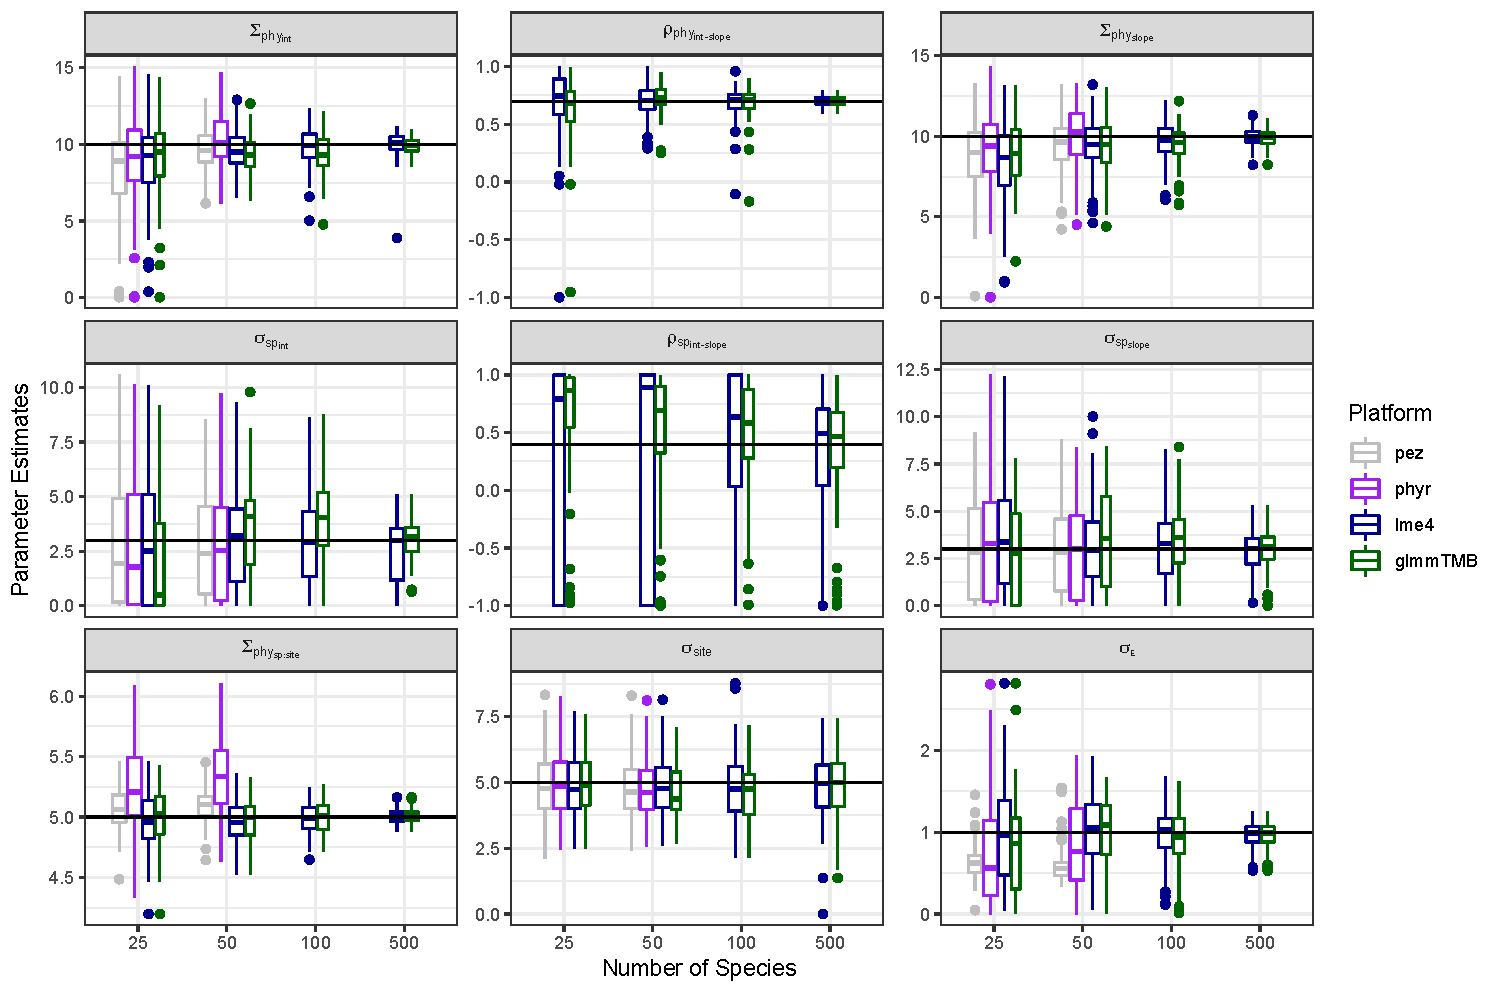
\includegraphics[scale=0.7,page=1]{./figure/msplot.pdf}
  \caption{Comparison of multi-group model parameter estimates. The horizontal line shows the true value of the parameters in the simulation model. Models capable of fitting all parameters (lme4 and glmmTMB) fit well for all parameters. \pkg{pez} and \pkg{phyr} estimates for n = 100, and 500 are not available because the models did not converge within 30 minutes. 
%    \bmb{need to work harder to match up colours across plots - colours corresponding to specific platforms are different in different plots because different subsets are included (use \code{scale\_colour\_manual} appropriately)}
  }
  \label{msplot}
\end{figure}
\end{center}
\begin{center}
\begin{figure}[H]
  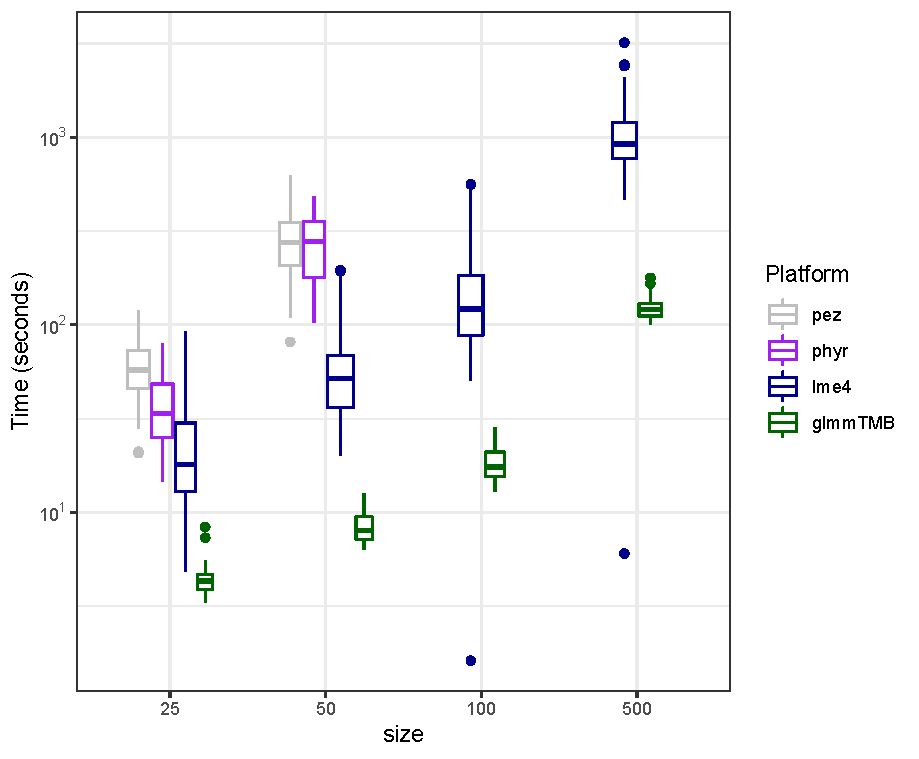
\includegraphics[scale=0.8]{./figure/mstime.pdf}
  \caption{Comparison of multi-group model computational speed.}
  \label{msplot_time}
\end{figure}
\end{center}
\begin{center}
\begin{figure}[H]
  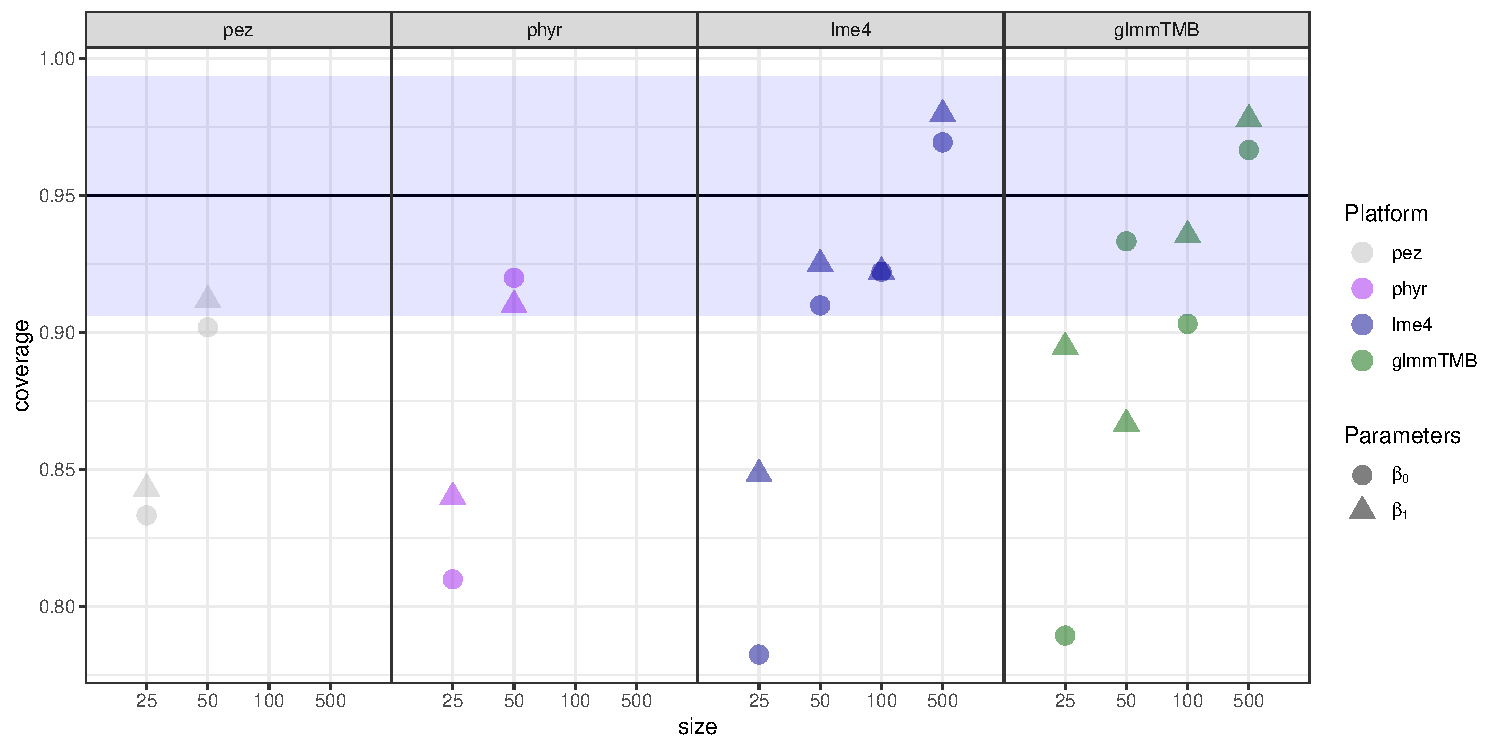
\includegraphics[scale=0.5]{./figure/mscoverage.pdf}
  \caption{Comparison of multi-group model coverage.}
  \label{msplot_coverage}
\end{figure}
\end{center}

In contrast, the multi-group model fits are much more similar across platforms (only the more powerful platforms can fit these models at all, and the fitting models are closer to the true simulation model).
Similar to the single-group fits, \pkg{lme4} and \pkg{glmmTMB} match the simulation model well and provide good estimates for all parameters except the correlation ($\sigma_{\mathrm{sp_{int-slope}}}$) for small numbers of species (i.e. n = 25 and 50).
The lack of correlations in \pkg{pez} and \pkg{phyr}'s statistical models does not appear to have a large effect on the estimates of the remaining parameters in the model but underestimates the residual standard deviation (Figure \ref{msplot}).

Although the parameter estimates are similar across platforms for the multi-group simulation fits, computational efficiency varies enormously across platforms and sample size.
For example, the new formulation is implemented in both \pkg{lme4} and \pkg{glmmTMB}, but \pkg{glmmTMB} is almost an order of magnitude faster than \pkg{lme4} for the cases studied here.
Comparing \pkg{glmmTMB} to \pkg{pez} and \pkg{phyr}, the median time for \pkg{glmmTMB} to fit 50 species model is $\approx$ 9 versus $\approx$ 200 seconds for \pkg{pez} and \pkg{phyr} respectively. 
\pkg{glmmTMB} takes $\approx$ 125 seconds to fit a 500-species model; it was not practical for us to fit 500-species models with \pkg{pez} and \pkg{phyr}, because computational speed scaled faster than linearly with sample size.
\pkg{glmmTMB} is almost an order of magnitude faster than \pkg{lme4}.

% \bmb{Can you put a lower bound on \pkg{pez}'s computation time? How long did you take to give up? How does it scale? can you either figure out from first principles
%   or (easier) do a brute-force series of increasing sample size and
%   compute a log-log regression of time vs sample size to find the
%   approximate power?}

\section*{Discussion}


% \bmb{say something about the implications of this [e.g. good enough for getting an overall impression of phylog. whatever-it-is but not enough for detailed description/inference about the evolutionary process?] (or maybe that should be saved for the Discussion?)}

We have simulated relatively complex models containing phylogenetic variation in both intercepts and slopes, as well as within-species variation that is quantifiable because we allow multiple observations per species.
These models are intrinsically more complex than some simple platforms for phylogenetic regression can handle, which may seem unfair; nevertheless, our models are certainly \emph{less} complex than evolutionary processes occurring in nature.
Our results show that models that cannot match the full ``simulation world'' perform poorly even for the parameters they do estimate; it is important to understand the limitations of these simpler, commonly used methods.

Even our relatively simple models can incorporate many layers of complexity --- e.g. multiple spatial grouping variables as well as correlated phylogenetic variation in the effects of several different traits and environmental variables on a focal trait.
In theory, as long as we have enough data and enough computational power, models that can incorporate more of the complexity will always describe a biological system better.
However, real applications are always data-constrained.
Deciding on a practically appropriate level of model complexity for a given
problem and data set is an
open and difficult general problem in statistical modeling, not just
in phylogenetic studies.
Should one use simple models that may be overly conservative or
risk overfitting by using more ambitious models?
How can one appropriately use the data themselves
to choose model complexity \citep{roberts_cross-validation_2016}?
What are the relative costs and benefits of using a step-down procedure
starting from the most complex possible model \citep{barr2013random},
choosing simpler models \emph{a priori} \citep{baayen2008mixed},
or using Bayesian approaches with regularizing priors \citep{hadfield2010mcmc}?

\subsection*{Incorporating different levels of variation}

% \bmb{I think you need a lot more here; what does a random slopes model mean? You have one sentence that says ``people should be thinking about random slopes''. Then you talk about correlation (which is a much more subtle/less important issue, I think).}

In classic GLMMs, random effects are used to handle group (or individual) level variation. 
In the simplest experimental design with continuous response observations in different levels of a discrete grouping variable, where the response may vary among levels of the grouping variable, fitting random intercepts are the ``go-to'' method to handle this variation.
The random intercept model controls the group effect in the response level by allowing different intercepts for each level of the grouping variable.
However, random effects can take more complicated forms as the experimental design becomes more complex.  
For example, imagine observing another continuous explanatory variable in the experimental design above, where the relationship of the response and the new explanatory variable may vary according to the grouping variable.
A random slopes model, which allows different slopes (the relationship between continuous variables) for each level of the grouping variable is most appropriate to handle this type of variation.
Random slopes models require appropriate observational or experimental designs (i.e., multiple measurements of traits and responses within each evolutionary group) and often require more data overall for reliable estimates, but they are relevant over a wide range of scenarios \citep{schielzeth2008conclusions, cleasby2015quantifying,ord2010adaptation}.
Neglecting random slopes can lead to biased fixed effect estimates with inadequate coverage and type I errors \citep{schielzeth2008conclusions} as shown in the simulations above.

% When analyzing relationships among species between traits, it is entirely plausible that change in the effect of predictor variables have on traits are changing with respect to different grouping of species or even in a phylogenetically correlated way (phylogenetic random slopes).
Nevertheless, it is hard to account for all forms of complexities and decide if when it is best to use phylogenetic random effects, simple grouping, or both. 
Optimal model complexity depends on experimental design and whether the data provides enough signal to estimate these different levels of variation, which can be strongly confounded.
For example, for experimental designs with single measurement per species, any method that can account for at least two sources of variation, such as Pagel's $\lambda$ will be sufficient. 
However, if multiple observations are available per species, then these simple methods may confound tip variation with residual variation.
In this case, multiple observations can summarized to a single measurement (for example, weighted-mean) per species to avoid confounding residual and tip variation.
This is equivalent to assuming homoscedasticity using inverse-variance weights for unbalanced datasets. 
Alternatively, when the within-species variance is actually of interest, accounting for within-species variation (i.e., adding species-level random effects in our example) can automatically handle multiple observations per species.

It may be easier to be conservative to include both (phylogenetic random effects and grouping random effects) of them but simplify the phylogenetic relationships (at the random slopes level) and think about the random-slopes model in a strictly hierarchical setting (i.e., estimating different slopes for each family, or taxon \citep{bunnefeld2012island}) - the PGLMM collapses to a standard random-slopes model. 

Another simplifying alternative is to be conservative to include both phylogenetic random effects and grouping random effects but simplify the phylogenetic relationships and think about the random-slopes model in a strictly hierarchical setting (i.e., estimating different slopes for each family, or taxon \citep{bunnefeld2012island}). 
However, this collapses phylogenetic structures to a standard random-slopes model. 
Users should be aware of two essential questions when fitting random-slope models: How much data do we need in order to practically estimate the random slopes? Are we making a mistake by ignoring random slopes \citep{schielzeth2008conclusions}? 
% However, in the PGLMM context, as long as there's variation in the predictor among tips, there will be variation among taxa at some level, so random-slopes models will (almost always) be \emph{theoretically} identifiable.

\subsection*{Extension and alternatives}

We have presented a range of classical phylogenetic comparative methods (i.e. phylogenetic least squares, linear and mixed models) to fit models that incorporate different levels of phylogenetic variation.
Even within this scope, there is additional room for exploration, such as phylogenetic multivariate response models; non-Brownian evolutionary processes such as the Ornstein-Uhlenbeck (OU) model which accounts for both selection and drift processes \citep{butler2004phylogenetic}); Bayesian approaches \citep{hadfield2010general}; and variable-rate model, where evolutionary parameters vary across the phylogeny.
However, the simple approach we developed here offers an efficient way to handle phylogenetic comparative analysis for a wide range of univariate, Brownian-motion evolutionary models. 
This approach can in principle be combined flexibly with any platforms that supports independent latent variables such as Stan.
More importantly, this implementation in \pkg{lme4} and \pkg{glmmTMB} allows users to fit phylogenetic mixed models to the fullest (large data, unbalanced species observations, complex random effects) and explore new ideas.

\section*{Authors’ contributions}

ML and BMB conceived the ideas and designed methodology; ML and BMB implemented the code in \pkg{lme4} and \pkg{glmmTMB}; ML ran all simulations; ML and BMB analyzed the results; ML wrote the first draft of the manuscript. All authors contributed critically to the drafts and gave final approval for publication.

\section*{Data Availability}

All codes are available at DOI:10.5281/zenodo.2639887.

% \section*{Conclusion}
% 
% We have presented a simple approach to fit phylogenetic mixed models that is both more efficient and statistically equivalent approach and comparison of classical PCM to simulated data. 
% Our approach is orders of magnitud faster than existing phylogenetic mixed models and it can easily combined with any statistical mixed model framework. 
% It is more flexible in fitting large phylogenies, large volumes of data, unbalanced data sets, and complex random effects such as slope correlations.

% \newpage
% 
% \section*{Supplements -- translation}
% 
% $1 \mid Sp_{phylo}$, $0 + X_{E} \mid Sp_{phylo}$ and $X_{E} \mid Sp_{phylo}$ means phylogenetically related have similar response,   
% 
% \begin{tabularx}{\textwidth}{|l|X|X|}
% \hline
% Formula & Statistics & Biology \\
% \hline
% $1 \mid Sp$ &
% random species intercept; variation within species in mean response across all factors &
% variation of how species respond \\
% \hline
% 
% $0 + X_{E} \mid Sp$ &
% random slope of environment factor within species; variation in coefficient within species for the environmental factor &
% variation of how species respond to the same environmental factor \\
% \hline
% 
% $1 + X_{E} \mid Sp$ &
% random slope of environmental factor within species with correlated intercept; variation in coefficient within species for the environmental factor with correlated mean response across all other factors &
% variation of how species respond in the same environmental factors and the correlation of the variation of how they respond in general \\
% \hline
% 
% $1 \mid Site:Sp $ &
% random variation in intercept among species within sites &
% variation of how species respond within sites \\
% \hline
% 
% $1 | Sp_{Phylo} $ &
% variation among species in mean response across all factors demonstrate phylogenetic signal &
% phylogenetically related species respond similarly \\
% \hline
% 
% $0 + X_{E} \mid Sp_{Phylo}$ &
% variation among species for environmental factors demonstrate phylogenetic signal &
% phylogenetically related species respond similar (share common response) to the same environmental factor \\
% \hline
% \end{tabularx}
%             
%             
%             
%             
%             
%                                                               
\singlespacing

\bibliography{phyloglmm}

\end{document}

